\documentclass[11pt,letterpaper]{article}
\usepackage{amssymb,amsmath}
\usepackage{mathrsfs}
\usepackage{epsfig}
\usepackage{anysize}
\usepackage{verbatim}
\usepackage{minted} %% Código
\usepackage[utf8]{inputenc}
\usepackage[spanish]{babel}
\usepackage{listings}
\usepackage{tikz} %% Para dibujar una lista simplemente ligada
\usetikzlibrary{calc,shapes.multipart,chains,arrows, babel}
\usepackage{forest}
\usepackage{caption}

%% Cambiar "listing" por "listado"
\renewcommand\listingscaption{Listado}
\renewcommand{\lstlistingname}{Listado}


\title{Implementación de Árboles Patricia en Coq}
\author{Víctor Zamora Gutiérrez}
\date{\today}
\begin{document}
\maketitle
\thispagestyle{empty}
\begin{abstract}
  \noindent La meta de este trabajo fue realizar una implementación de árboles Patricia en Coq. Para esta implementación, era deseable demostrar que las operaciones principales funcionaban; con esto nos referimos a las operaciones de inserción y unión de árboles. La meta se logró de manera satisfactoria para la operación de inserción. Para la de unión, hubieron algunos problemas que evitaron que demostráramos propiedades sobre ella, pero al menos se demostró que la función utiliza recursión bien fundada.
\end{abstract}
\section{Introducción}
\noindent Los Árboles Patricia\cite{} son estructuras de datos que funcionan como diccionarios con llaves enteras. Son atractivos debido a la sencillez con la que se implementan en lenguajes funcionales y debido a su eficiencia. La idea básica es que se tiene un árbol en el que el $0$ representa ``izquierda'' y el $1$ representa ``derecha''. Por ejemplo, en el árbol de la figura~\ref{fig:Pat}, el elemento $y$ tiene llave $4$, pues $4=100$ y para llegar a $y$ tenemos que tomar el camino izquierda-izquierda-derecha (leyendo el número de adelante hacia atrás). Como podemos notar, los elementos siempre estarán en hojas de los árboles.

\begin{figure}[h]
\label{fig:Pat}
\caption{Figura obtenida en \cite{}}
\centering
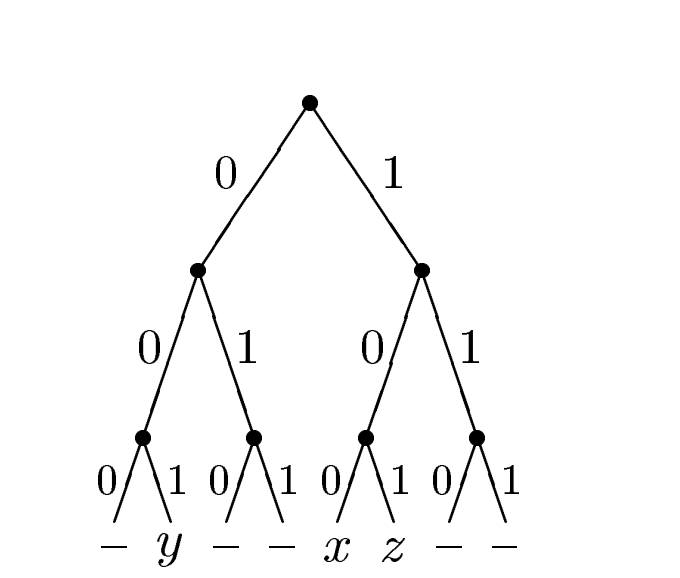
\includegraphics[ width=0.5\textwidth]{img/pat1}
\end{figure}

Por supuesto, si los árboles Patricia estuvieran implementados como el de la figura~\ref{fig:Pat}, no serían muy útiles, pues las búsquedas tomarían tiempo lineal sobre el tamaño de las llaves, lo cual no es muy óptimo. Por esto, de esta idea básica se obtienen varias optimizaciones para crear una estructura de datos eficiente, de las cuales hablaremos más adelante.

En este trabajo se decidió hacer una implementación de árboles Patricia en Coq. Se comenzó desde lo más básico, que son los tries binarios (estructuras de la figura~\ref{fig:Pat}) hasta llegar a la estructura final. Para la estructura final, se implementaron las operaciones de búsqueda, inserción y unión, de las cuales también hablaremos más adelante. Además se verificó el funcionamiento de la inserción con respecto a búsquedas. Para la unión no se verificó nada debido a la forma en la que tuvo que definirse; sin embargo se logró definir a pesar de que utiliza recursión distinta a la que se trabajó con Coq a lo largo del semestre.

\section{Estructura del Proyecto}

\noindent El proyecto está dividido en dos tipos de archivos: de definiciones y de proposiciones. Los archivos de definiciones son:

\begin{itemize}
\item \texttt{Defs\_Bin.v} - Contiene definiciones de funciones sobre números binarios.
\item \texttt{Defs\_Misc.v} - Contiene definiciones miscelaneas.
\item \texttt{Defs\_Patricia.v} - Contiene definiciones de árboles Patricia.
\item \texttt{Defs\_Trie.v} - Contiene definiciones de tries binarios y sus optimizaciones.
\end{itemize}

Los archivos de proposiciones son:

\begin{itemize}
\item \texttt{Props\_Bin.v} - Contiene proposiciones de funciones sobre números binarios.
\item \texttt{Props\_Misc.v} - Contiene proposiciones miscelaneas.
\item \texttt{Props\_Patricia.v} - Contiene proposiciones de árboles Patricia.
\item \texttt{Props\_Trie.v} - Contiene proposiciones de tries binarios y sus optimizaciones.
\end{itemize}

Para que el proyecto funcione correctamente, es necesario compilar cada archivo por separado. Esto se puede hacer desde CoqIde con Compile $\rightarrow$ Compile buffer.

Se utilizó la versión \textbf{8.13} de CoqIde. No se garantiza el funcionamiento del proyecto en versiones anteriores o posteriores de CoqIde.

\section{Herramientas}

\noindent Para el desarrollo del proyecto, utilizamos algunas bibliotecas auxiliares de Coq. La más importante de estas fue la biblioteca \texttt{BinNat}\cite{} que define a los números naturales en binario. Esta biblioteca se usó para definir las llaves y la estructura general de los árboles. Además de esta, utilizamos las siguientes bibliotecas:
\begin{itemize}
\item \texttt{BinPos} - Para enteros positivos binarios (naturales sin cero).
\item \texttt{Lia} - Para demostrar propiedades de operaciones aritméticas.
\item \texttt{Bool.Bool} - Para propiedades sobre el tipo \texttt{Bool} de Coq.
\end{itemize}

\section{Desarrollo de árboles Patricia}\label{section:desarrollo}

\subsection{Tries binarios}

\noindent Decidimos basarnos completamente en\cite{} para el desarrollo del proyecto. Esto implicó una optimización gradual del trie binario hasta llegar a árboles Patricia.

El trie binario es la estructura de datos de la figura~\ref{fig:Pat}. Básicamente es un árbol binario en el que cada arista está etiquetada con $0$ o $1$, dependiendo de si es arista izquierda o derecha. Los nodos internos no contienen ninguna información; son las hojas quienes contienen a los elementos del árbol. Nuestra definición del trie binario se encuentra en el listado~\ref{lst:trieBin}.

\begin{listing}[H]
  \inputminted{coq}{src/trie.v}
  \caption{Definición de trie binario}
  \label{lst:trieBin}
\end{listing}

La búsqueda en trie binario es sencilla. Para buscar una llave $x$ simplemente vemos si es par o impar. Si es par, buscamos por el lado izquierdo y si es impar buscamos por el derecho. Dividimos la llave entre dos y continuamos el proceso hasta llegar a una hoja. La función de búsqueda está en el listado~\ref{lst:lookup}.

\begin{listing}[H]
  \inputminted{coq}{src/lookup.v}
  \caption{Búsqueda en un trie binario}
  \label{lst:lookup}
\end{listing}


\subsection{Primera Optimización}
\noindent La primera optimización que se hace para los tries binarios es colapsar a dos subárboles vacíos en un solo árbol. Esto para decrementar el tamaño del árbol. Dicha optimización se logra por medio de un \textit{constructor inteligente}. La idea de los constructores inteligentes es que en lugar de utilizar el constructor \texttt{trie} del listado~\ref{lst:trieBin}, utilizaremos únicamente el constructor inteligente para construir nuestros árboles. El constructor inteligente se enecuentra en el listado~\ref{lst:smart1}.

\begin{listing}[H]
  \inputminted{coq}{src/smart1.v}
  \caption{Primera optimización de los tries binarios}
  \label{lst:smart1}
\end{listing}

\subsection{Segunda Optimización}
\noindent La segunda optimización sale de la siguiente consideración: supongamos que tenemos un árbol cuyo único elemento es una hoja y el resto de sus subárboles son vacíos. En la figura~\ref{fig:arbol_chafa} podemos ver un árbol así. Este árbol tiene un solo elemento; sin embargo, tenemos que recorrerlo todo para encontrar este elemento. Esto no tiene mucho sentido, y de aquí surge la idea de colapsar este tipo de árboles en un solo nodo. Para lograr esto, se usó la optimización del listado~\ref{lst:opt2}. Este listado contiene otro constructor inteligente que, al encontrar una hoja junto a un árbol vacío, colapsa el árbol vacío con la hoja.

\begin{figure}[h]
  \caption{Árbol con una sola hoja}
  \label{fig:arbol_chafa}
   \centering
  \begin{tikzpicture}
    \tikzstyle{every child node}=[circle,draw]
    \node(Root)[circle, draw]{}
    child[missing]{}
    child{node[circle,draw]{}
      child[missing]{}
      child{node[circle,draw]{}
        child[missing]{}
        child{node[circle,draw]{$n$} edge from parent node[right,draw=none] {$1$}}
        edge from parent node[right,draw=none] {$1$}
      }
      edge from parent node[right,draw=none] {$1$}
    };
  \end{tikzpicture}
\end{figure}

\begin{listing}[H]
  \inputminted{coq}{src/smart2.v}
  \caption{Segunda optimización de los tries binarios}
  \label{lst:opt2}
\end{listing}

Para que esta optimización funcionara, tuvimos que modificar la estructura de árbol para que las hojas guardaran un prefijo de su llave. La nueva estructura de árbol está en el listado~\ref{lst:prefix}.

\begin{listing}[H]
  \inputminted{coq}{src/prefix.v}
  \caption{Árboles cuyas hojas guardan una llave}
  \label{lst:prefix}
\end{listing}

Observemos que los prefijos que guardan las hojas son de tipo \texttt{N}. Este es el tipo para números binarios en Coq.

Después de realizar esta optimización, hay que modificar ligeramente la función de búsqueda para que al llegar a una hoja, revise que el prefijo de la hoja sea igual al elemento que busca.

\subsection{Tercera optimización}

\noindent Una alternativa a la optimización anterior es que en lugar de que las hojas guarden un prefijo de su llave, guarden la llave completa. Así, en la función de búsqueda ya no tenemos que descartar bits (o equivalentemente, dividir). Para que esto funcione, es necesario que los nodos guarden el bit sobre el que se dividen. Lo que esto quiere decir es que cada nodo guarda su profundidad, y así la función de búsqueda solo tiene que revisar el bit correspondiente a la profundidad del nodo.

Como guardar la profundidad complica los cálculos de buscar el bit correspondiente, en la práctica lo que se hace es guardar un entero binario con un solo bit prendido, y revisar dicho bit en la llave buscada.

Para esto, definimos la nueva estructura dada por el listado~\ref{lst:trie3}. La nueva función de búsqueda se encuentra en el listado~\ref{lst:lookup3}. La función \texttt{zeroBit} nos dice si el bit prendido de \texttt{m} está apagado en \texttt{key}. Podemos verla en el listado~\ref{lst:zeroBit}.

\begin{listing}[H]
  \inputminted{coq}{src/trie3.v}
  \caption{Estructura de datos definida de acuerdo a la nueva optimización}
  \label{lst:trie3}
\end{listing}

\begin{listing}[H]
  \inputminted{coq}{src/lookup3.v}
  \caption{Nueva función de búsqueda}
  \label{lst:lookup3}
\end{listing}

\begin{listing}[H]
  \inputminted{coq}{src/zeroBit.v}
  \caption{Función que revisa si un bit está apagado}
  \label{lst:zeroBit}
\end{listing}

\subsection{Árboles Patricia}
\noindent Nos encontramos muy cerca de los árboles Patricia. Solo nos falta hacer una optimización más a nuestros tries binarios.

El caso que nos falta optimizar es en el que todas las hojas tienen un prefijo en común. En este caso, la búsqueda recorrerá los bits del prefijo uno a la vez hasta llegar a un nodo del que salen todas las hojas. Esto se puede optimizar si nos evitamos recorrer los bits del prefijo. Como sabemos que hay un solo prefijo útil en el subárbol, podemos colapsar ese camino. La estructura bajo esta optimización es a lo que llamamos árbol Patricia. De nuevo, hay que cambiar nuestra estructura de datos, ahora para que los nodos internos guarden el prefijo que se ha leído hasta el momento. La nueva estructura está en el listado~\ref{lst:patricia}. Un ejemplo de un árbol Patricia está en la figura~\ref{fig:Patricia}.

\begin{listing}[H]
  \inputminted{coq}{src/patricia.v}
  \caption{Definición de árboles Patricia}
  \label{lst:patricia}
\end{listing}

\begin{figure}[h]
\label{fig:Patricia}
\caption{Figura obtenida en \cite{} y modificada posteriormente. Los números en rojo representan los prefijos y bits que se guardan en cada nodo.}
\centering
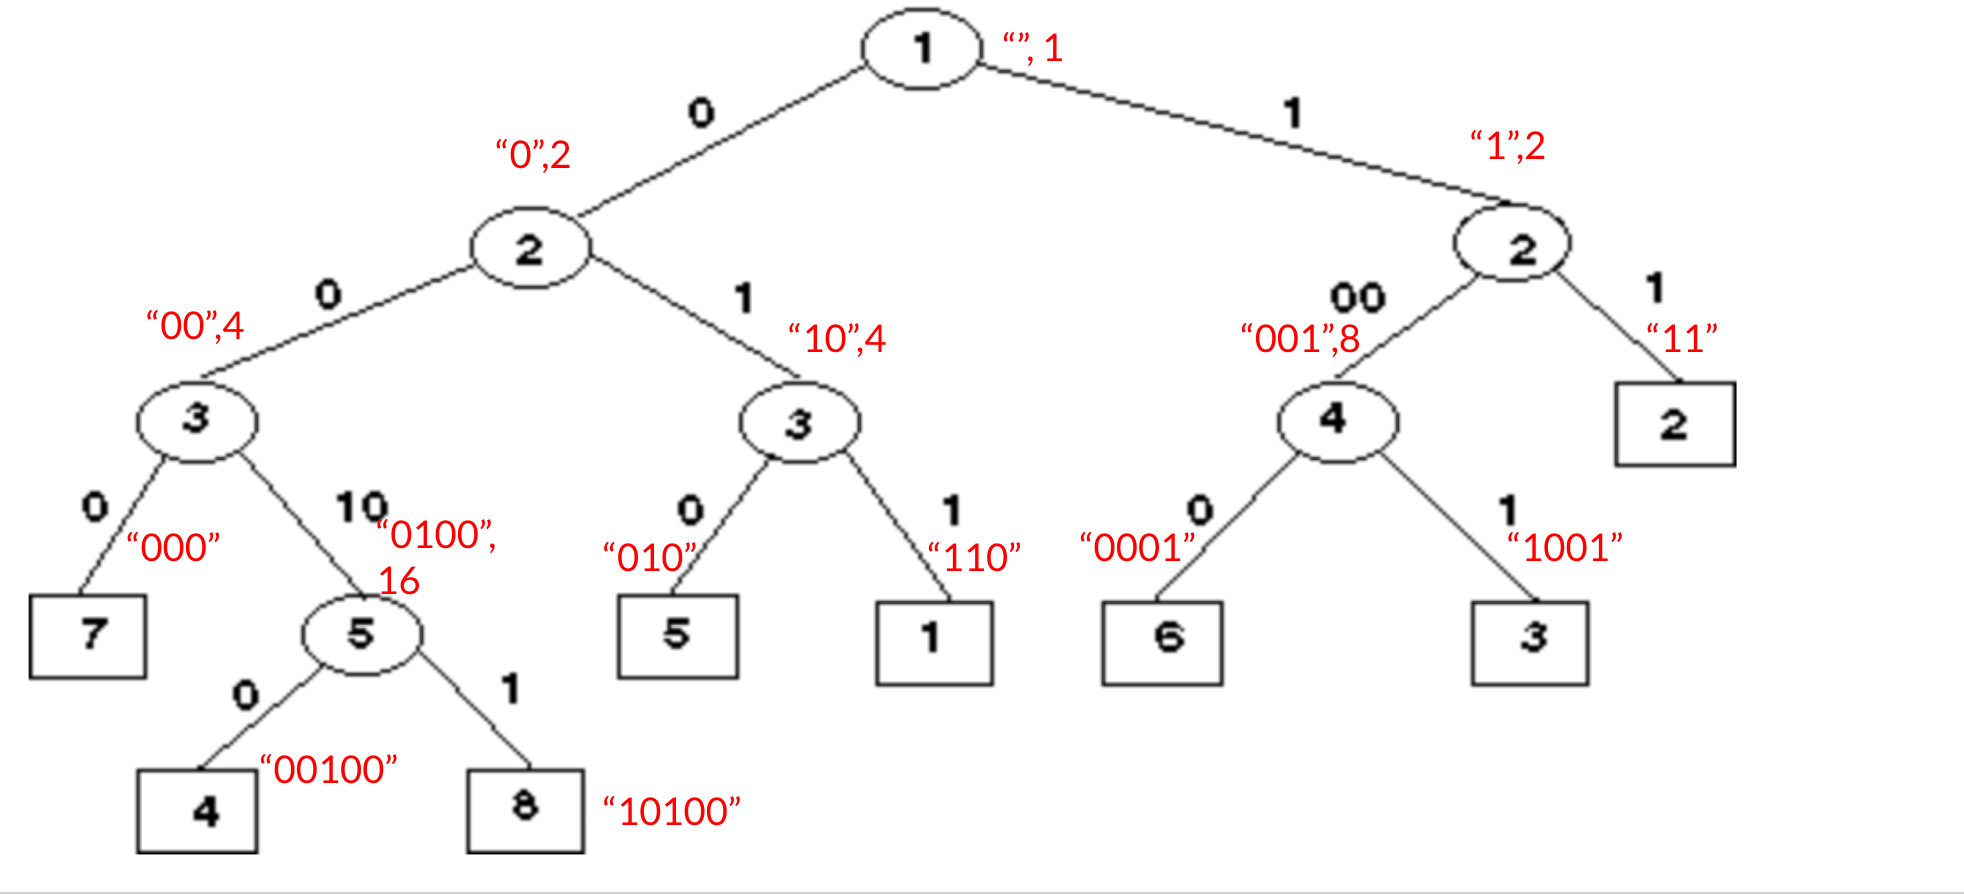
\includegraphics[ width=0.5\textwidth]{img/pat2}
\end{figure}

\section{Metas del proyecto}
\noindent Se plantearon las siguientes metas de manera concreta:
\begin{enumerate}
\item Definir tries binarios. \label{itm:tries}
\item Definir árboles Patricia.\label{itm:pat}
\item Definir la operación de búsqueda en árboles Patricia.\label{itm:lookup}
\item Definir la operación de inserción en árboles Patricia. \label{itm:insert}
\item Demostrar corrección de inserción con respecto a búsquedas.\label{itm:dem1}
\item Definir operación de unión de dos árboles Patricia.\label{itm:defUnion}
\item Demostrar corrección de la unión. \label{itm:union}
\item Definir una operación alternativa de búsqueda más óptima.\label{itm:busqueda2}
\item Demostrar equivalencia entre ambas operaciones de búsqueda.\label{itm:prueba2} 
\end{enumerate}
\section{Resultados}
\noindent Todas las metas se lograron excepto por la meta~\ref{itm:union}. Las metas~\ref{itm:tries} y~\ref{itm:pat} se mencionaron en la sección~\ref{section:desarrollo}, por lo que únicamente mencionaremos los resultados de las demás metas.
\subsection{Meta~\ref{itm:lookup}}
\noindent La implementación de la función de búsqueda se puede ver en el listado~\ref{lst:busqueda} y es practicamente una copia de la que se encuentra en\cite{}. La función \texttt{matchPrefix} se encarga de ver si, dados tres enteros $k$, $p$ y $m$, $k$ y $p$ coinciden en los primeros $\log_2m$ bits.

\begin{listing}[H]
  \inputminted{coq}{src/busqueda.v}
  \caption{Función de búsqueda para árboles Patricia}
  \label{lst:busqueda}
\end{listing}

La función \texttt{zeroBit} nos dice, para dos números $k$ y $m$, si el $\log_2m$-ésimo bit de $k$ es $0$.

La función \texttt{mask} es una máscara como en la definición usual, salvo porque en lugar de recibir un número de la forma $2^n-1$, recibe uno de la forma $2^n$ y saca el predecesor de este.

Las funciones \texttt{matchPrefix}, \texttt{zeroBit} y \texttt{mask} están en el listado~\ref{lst:bin}.

\begin{listing}[H]
  \inputminted{coq}{src/bin.v}
  \caption{Definiciones de operaciones binarias en Coq}
  \label{lst:bin}
\end{listing}

\subsection{Meta~\ref{itm:insert}}
\noindent La función de inserción también se sacó de\cite{} y está en el listado~\ref{lst:insert}. 

\begin{listing}[H]
  \inputminted{coq}{src/insert.v}
  \caption{Función de inserción}
  \label{lst:insert}
\end{listing}

\subsection{Meta~\ref{itm:dem1}}
\noindent Se logró satisfactoriamente demostrar la correción de la inserción con respecto a la búsqueda. Se demostró la corrección en dos casos: cuando el elemento insertado no estaba previamente en el árbol y cuando sí estaba ahí.

\subsection{Meta~\ref{itm:defUnion}}
\noindent Esta meta se logró satisfactoriamente, aunque no de la manera que se esperaba. Debido a que la función de unión que se obtuvo del artículo no era recursiva simple, esta no se pudo definir usando \texttt{Fixpoint}. Investigando en internet se encontró un conjunto de tácticas denominadas \texttt{Program}\cite{}, en donde se encuentra el comando \texttt{Program Fixpoint}, a partir del cual se pueden definir funciones con recursiones más complicadas que las aceptadas por \texttt{Fixpoint}.

Para definir una función con \texttt{Program Fixpoint}, basta con hacer lo siguiente:

\begin{enumerate}
\item Definir una medida que decrezca con cada paso de la recursión. En nuestro caso, utilizamos el número de nodos de los árboles como medida.
\item Probar que la recursión termina.
\end{enumerate}

La definición de nuestra función con \texttt{Program Fixpoint} está en el listado~\ref{lst:pf}. Tras definirla, tuvimos que probar una serie de obligaciones para convencer al asistente de que la recursión terminaba.

\begin{listing}[H]
  \inputminted{coq}{src/ProgramFixpoint.v}
  \caption{Función de inserción}
  \label{lst:pf}
\end{listing}


Este programa que a la vista de cualquier programador experimentado parece sencillo, en realidad causa dificultades para sistemas tan rigurosos como Coq. Es una de las formas en que podemos darnos cuenta de que la verificación formal aún tiene mucho hacia dónde crecer.

\subsection{Meta~\ref{itm:union}}
\noindent Esta meta no se logró debido a la poca experiencia con el uso de \texttt{Program}.

Al intentar demostrar propiedades con respecto a la función \texttt{merge}, nos topamos con que las definiciones escritas con \texttt{Program Fixpoint} no se pueden simplificar. Esto nos dejó como opción el desdoblar la definición. Desgraciadamente, parece que no era la forma correcta de resolver el problema, pues el desdoblar la definición nos lo que está en el listado~\ref{lst:ilegible}: un programa ilegible.

  \inputminted{coq}{src/ilegible.v}
  \captionof{listing}{Código ilegible\label{lst:ilegible}}
  \subsection{Metas~\ref{itm:busqueda2} y~\ref{itm:prueba2}}
  \noindent Como no logramos la meta~\ref{itm:union}, decidimos cambiarla por otra tarea. En el artículo se menciona una definición alternativa de \texttt{lookup} que es un poco más eficiente. La tarea que nos dimos fue definir esta función y probar su equivalencia con la otra función de búsqueda. La definición de la función está en el listado~\ref{lst:lookup2}.

  \begin{listing}[H]
  \inputminted{coq}{src/lookup2.v}
  \caption{Función de búsqueda más eficiente}
  \label{lst:lookup2}
\end{listing}


  La meta se logró de manera satisfactoria, aunque por desgracia, tuvimos que admitir algunos lemas sobre números binarios por falta de tiempo. Considerando que nuestro archivo de propiedades sobre números binarios ya sobrepasa las $500$ líneas, es de nuestra opinión que haber demostrado toda las propiedades habría sido un proyecto por sí mismo; por esto, nos sentimos satisfechos a pesar de no haber demostrado todo.

  \section{Conclusiones}
  \noindent Se lograron satisfactoriamente la mayoría de las metas. Para un futuro, sería bueno aprender a utilizar \texttt{Program} y terminar las demostraciones de números binarios; aún así, el trabajo que se hizo está bastante completo.

  Con este proyecto nos quedamos con el aprendizaje de que realizar un proyecto de un ejemplo real, por más pequeño que parezca, es una gran tarea. La verificación formal está en pañales y con buena razón; es difícil avanzar en el trabajo. Sin embargo, creemos que poco a poco, mientras haya dedicación e ideas, habrá un futuro en el que el área de verificación formal prolifere.

\nocite{*}
 \bibliographystyle{IEEEtran}
 \bibliography{Proyecto}
 
\end{document}
